
\chapter{Definitions of Tree}
\lbl{app:trees}%
%
\index{tree!graph@as graph|(}%
%
\index{graph!tree@of tree|(}
%

\chapterquote{%
I met this guy\\
\makebox[0em][l]{and he looked like he might have been a hat-check clerk}\\
at an ice rink\\
which in fact\\
he turned out to be}{%
Laurie Anderson~\cite{Laurie}}


\noindent
Trees appear everywhere in higher-dimensional algebra.  In this text they
were defined in a purely abstract way~(\ref{eg:opd-of-trees}): $\tr$ is the
free plain operad on the terminal object of $\Set^\nat$, and an $n$-leafed
tree is an element of $\tr(n)$.  But for the reasons laid out at the
beginning of~\ref{sec:trees}, I give here a `concrete', graph-theoretic,
definition of (finite, rooted, planar) tree and sketch a proof that it is
equivalent to the abstract definition.

\section{The equivalence}

The main subtlety is that the trees we use are not quite finite graphs in
the usual sense: some of the edges have a vertex at only one of their ends.
(Recall from~\ref{eg:opd-of-trees} that in a tree, an edge with a free end
is not the same thing as an edge ending in a vertex.)  This suggests the
following definitions.

\begin{defn}
\item A (planar) \demph{input-output graph}%
%
\index{graph!input-output}
%
(Fig.~\ref{fig:comb-graphs}(a))
consists of
%
\begin{itemize}
\item a finite set $V$ (the \demph{vertices})
\item a finite set $E$ (the \demph{edges}), a subset $I \sub E$ (the
\demph{input edges}), and an element $o \in E$ (the \demph{output edge})
\item a function $s: E\without I \go V$ (\demph{source}) and a function $t:
E\without \{o\} \go V$ (\demph{target})
\item for each $v \in V$, a total order $\leq$ on $t^{-1}\{v\}$.
\end{itemize}
%
\end{defn}
%
\begin{figure}
\centering
\setlength{\unitlength}{1mm}
\begin{picture}(105,50)(0,-5)
\cell{0}{0}{bl}{%
\begin{picture}(50,45)
\cell{0}{0}{bl}{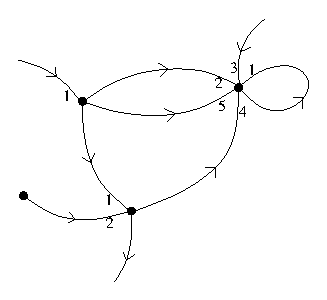
\includegraphics{iograph.eps}}
\cell{20}{3}{c}{o}
\cell{5}{38}{c}{i_1}
\cell{38}{45}{t}{i_2}
\end{picture}}
%
\cell{25}{-5}{b}{\textrm{(a)}}
%
\cell{62}{0}{bl}{%
\begin{picture}(43,45)(-1,0)
\cell{0}{0}{bl}{\includegraphics{combitree.eps}}
\cell{26}{4}{l}{o}
\cell{1}{41}{c}{i_1}
\cell{20}{41}{c}{i_2}
\cell{26}{27}{l}{i_3}
\end{picture}}
%
\cell{83.5}{-5}{b}{\textrm{(b)}}
\end{picture}
% \hand{50}{26}
\caption{(a) Input-output graph with 4 vertices and 2 input edges $i_1,
i_2$, (b) combinatorial tree with 4 vertices and 3 input edges $i_1, i_2,
i_3$.  In both, the numbers indicate the order on the edges arriving at
each vertex.}
\label{fig:comb-graphs}
\end{figure}
%
We write $v \goby{e}$ to mean that $e$ is a non-input edge with $s(e) = v$,
and similarly $\goby{e} v'$ to mean that $e$ is a non-output edge with
$t(e) = v'$, and of course \mbox{$v \goby{e} v'$} to mean that $e$ is a
non-input, non-output edge with $s(e) = v$ and $t(e) = v'$.

A tree is roughly speaking a connected, simply connected graph, and the
following notion of path allows us to express this.  

\begin{defn}
A \demph{path}%
%
\index{path!graph@in graph}
%
from a vertex $v$ to an edge $e$ in an input-output graph is
a diagram
\[
v= v_1 \goby{e_1} v_2 \goby{e_2} 
\ \cdots \ 
\goby{e_{l-1}} v_l \goby{e_l = e}
\]
in the graph.  That is, a path from $v$ to $e$ consists of
%
\begin{itemize}
\item an integer $l\geq 1$
\item a sequence $(v_1, v_2, \ldots, v_l)$ of vertices with $v_1=v$
\item a sequence $(e_1, \ldots, e_{l-1}, e_l)$ of edges with $e_l=e$
\end{itemize}
%
such that
\[
v_1 = s(e_1), \ 
t(e_1) = v_2 = s(e_2), \ 
\ldots, \ 
t(e_{l-1}) = v_l = s(e_l)
\]
and all of these sources and targets are defined.
\end{defn}

\begin{defn}
A \demph{combinatorial tree}%
%
\index{tree!combinatorial}
%
is an input-output graph such that for every
vertex $v$, there is precisely one path from $v$ to the output edge.
\end{defn}
%
Fig.~\ref{fig:comb-graphs}(b) shows a combinatorial tree.  The ordering of
the edges arriving at each vertex encodes the planar embedding.  `Tree' is
an abbreviation for `finite, rooted,%
%
\index{root of tree}
%
planar tree'.  If we were doing
symmetric operads then we would use non-planar trees, if we were doing
cyclic operads then we would use non-rooted trees, and so on.

A combinatorial tree is essentially the same thing as a tree in our sense,
where `essentially the same thing' refers to the obvious notion of
isomorphism between combinatorial trees.  We write $\fcat{combtr}(n)$ for
the set of isomorphism classes of combinatorial trees with $n$ input edges.

\begin{propn}
For each $n\in\nat$, there is a canonical bijection $\tr(n) \iso
\fcat{combtr}(n)$. 
\end{propn}

With a little more work we could define an operad structure on
$(\fcat{combtr}(n))_{n\in\nat}$ and turn the proposition into the stronger
statement that the operads $\tr$ and $\fcat{combtr}$ are isomorphic.  With
more work still we could define maps between combinatorial trees and
so define a \Cat-operad $\fcat{COMBTR}$ in which $\fcat{COMBTR}(n)$ is the
category of $n$-leafed combinatorial trees; then we could prove that this
\Cat-operad is equivalent to the \Cat-operad $\TR$.

\begin{prooflike}{Sketch proof}
The strategy is to define functions 
\[
\tr(n) \oppair{\Phi}{\Psi} 
\{ \textrm{combinatorial trees with } n \textrm{ input edges} \}
\]
for each $n\in\nat$, such that if $G \iso G'$ then $\Psi(G) =
\Psi(G')$, and such that $\Psi(\Phi(\tau)) = \tau$ and $\Phi(\Psi(G))
\iso G$ for each tree $\tau$ and combinatorial tree $G$.  The proposition
follows.  The definition of $\Phi(\tau)$ is by induction on the structure
of the tree $\tau$, and the definition of $\Psi(G)$ is by induction on the
number of vertices of the combinatorial tree $G$.  All the details are
straightforward. 
% 
\done
\end{prooflike}



\begin{notes}

Some pointers to the literature on trees can be found in the Notes to
Chapter~\ref{ch:opetopic}.%
%
\index{tree!graph@as graph|)}%
%
\index{graph!tree@of tree|)}
% 



\end{notes}
